\subsection{Normal VS Abnormal VS Artifact Model}
One of the primary concerns in applying machine learning models to the medical field is the potential 
consequence of misclassifying abnormal conditions as normal. Specifically, in the case of heartbeats, 
misclassifying an abnormal heartbeat as normal can have severe clinical implications. Therefore, 
our focus shifts from achieving the highest overall accuracy to minimizing the false positive rate (FPR) 
for the normal class. This approach ensures that fewer abnormal heartbeats are incorrectly classified as 
normal, thereby enhancing patient safety and diagnostic reliability.

\subsubsection{Methodology}
To effectively address the classification challenge, we categorized the heartbeats into three classes: 
normal, abnormal, and artifact, with the latter encompassing extrasystoles, murmurs, and extrahls. 
We then selected models from the previous section, prioritizing those with a low risk score. 
The features utilized were the filtered ones, and no class balancing was necessary since the classes 
were inherently balanced.

Each model was trained on 80\% of the dataset and tested on the remaining 20\%. 
The evaluation metrics included the ROC curve, macro F1 score, and balanced accuracy.


\subsubsection{Results}
The initial evaluation is presented using the ROC curves for all models. To address 
the three-class problem, we employed the one-vs-rest strategy, comparing each class against 
the others. Figure \ref{fig:ROC_normVSrest_allmodels} displays the ROC curves for the normal 
class versus the other classes across all models.

\begin{figure}[H]
    \centering
    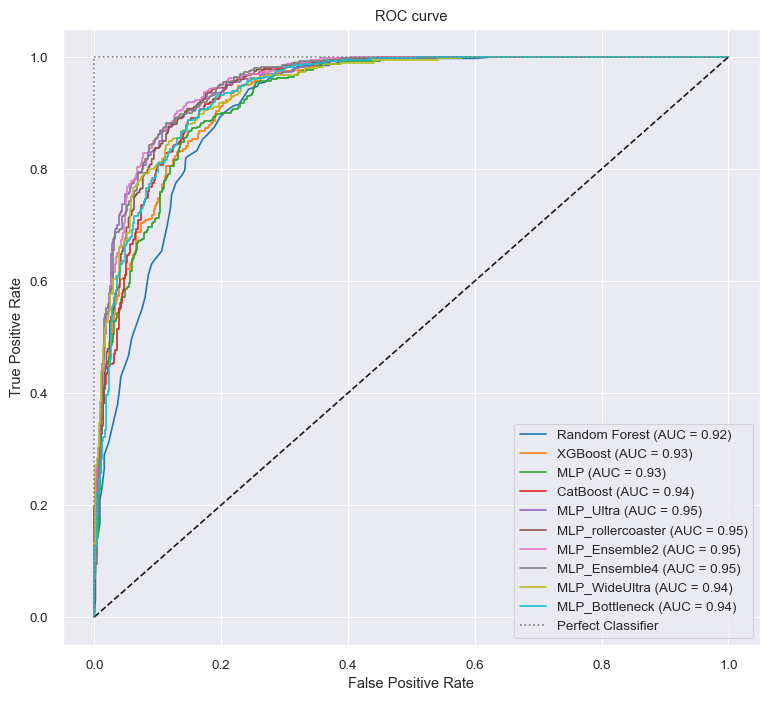
\includegraphics[width=1\columnwidth]{./images/ROC_normVSrest_allmodels.png}
    \caption{ROC curves for the normal class against the rest of the classes across all models.}
    \label{fig:ROC_normVSrest_allmodels}
\end{figure}

The results, indicated by the AUC values, show that the MLP model outperformed the others. 
Specifically, \textit{MLP\_Ensemble5} achieved the highest AUC value of 0.96, followed 
by \textit{MLP\_Ultra}, \textit{MLP\_Rollercoaster}, \textit{MLP\_Ensemble2}, 
and \textit{MLP\_Ensemble4}, all with an AUC of 0.95. \textit{MLP\_Ensemble5} also 
had the highest MCC value in the multiclass classification task, confirming its superior performance.

To further analyze model performance, we selected four FPR levels (1\%, 5\%, 10\%, 20\%) and 
calculated the corresponding TPR. The consolidated results are shown in 
Figure \ref{fig:normVSrest_all}, with detailed results for each FPR case available in the appendix.

\begin{figure*}[htpb]
    \centering
    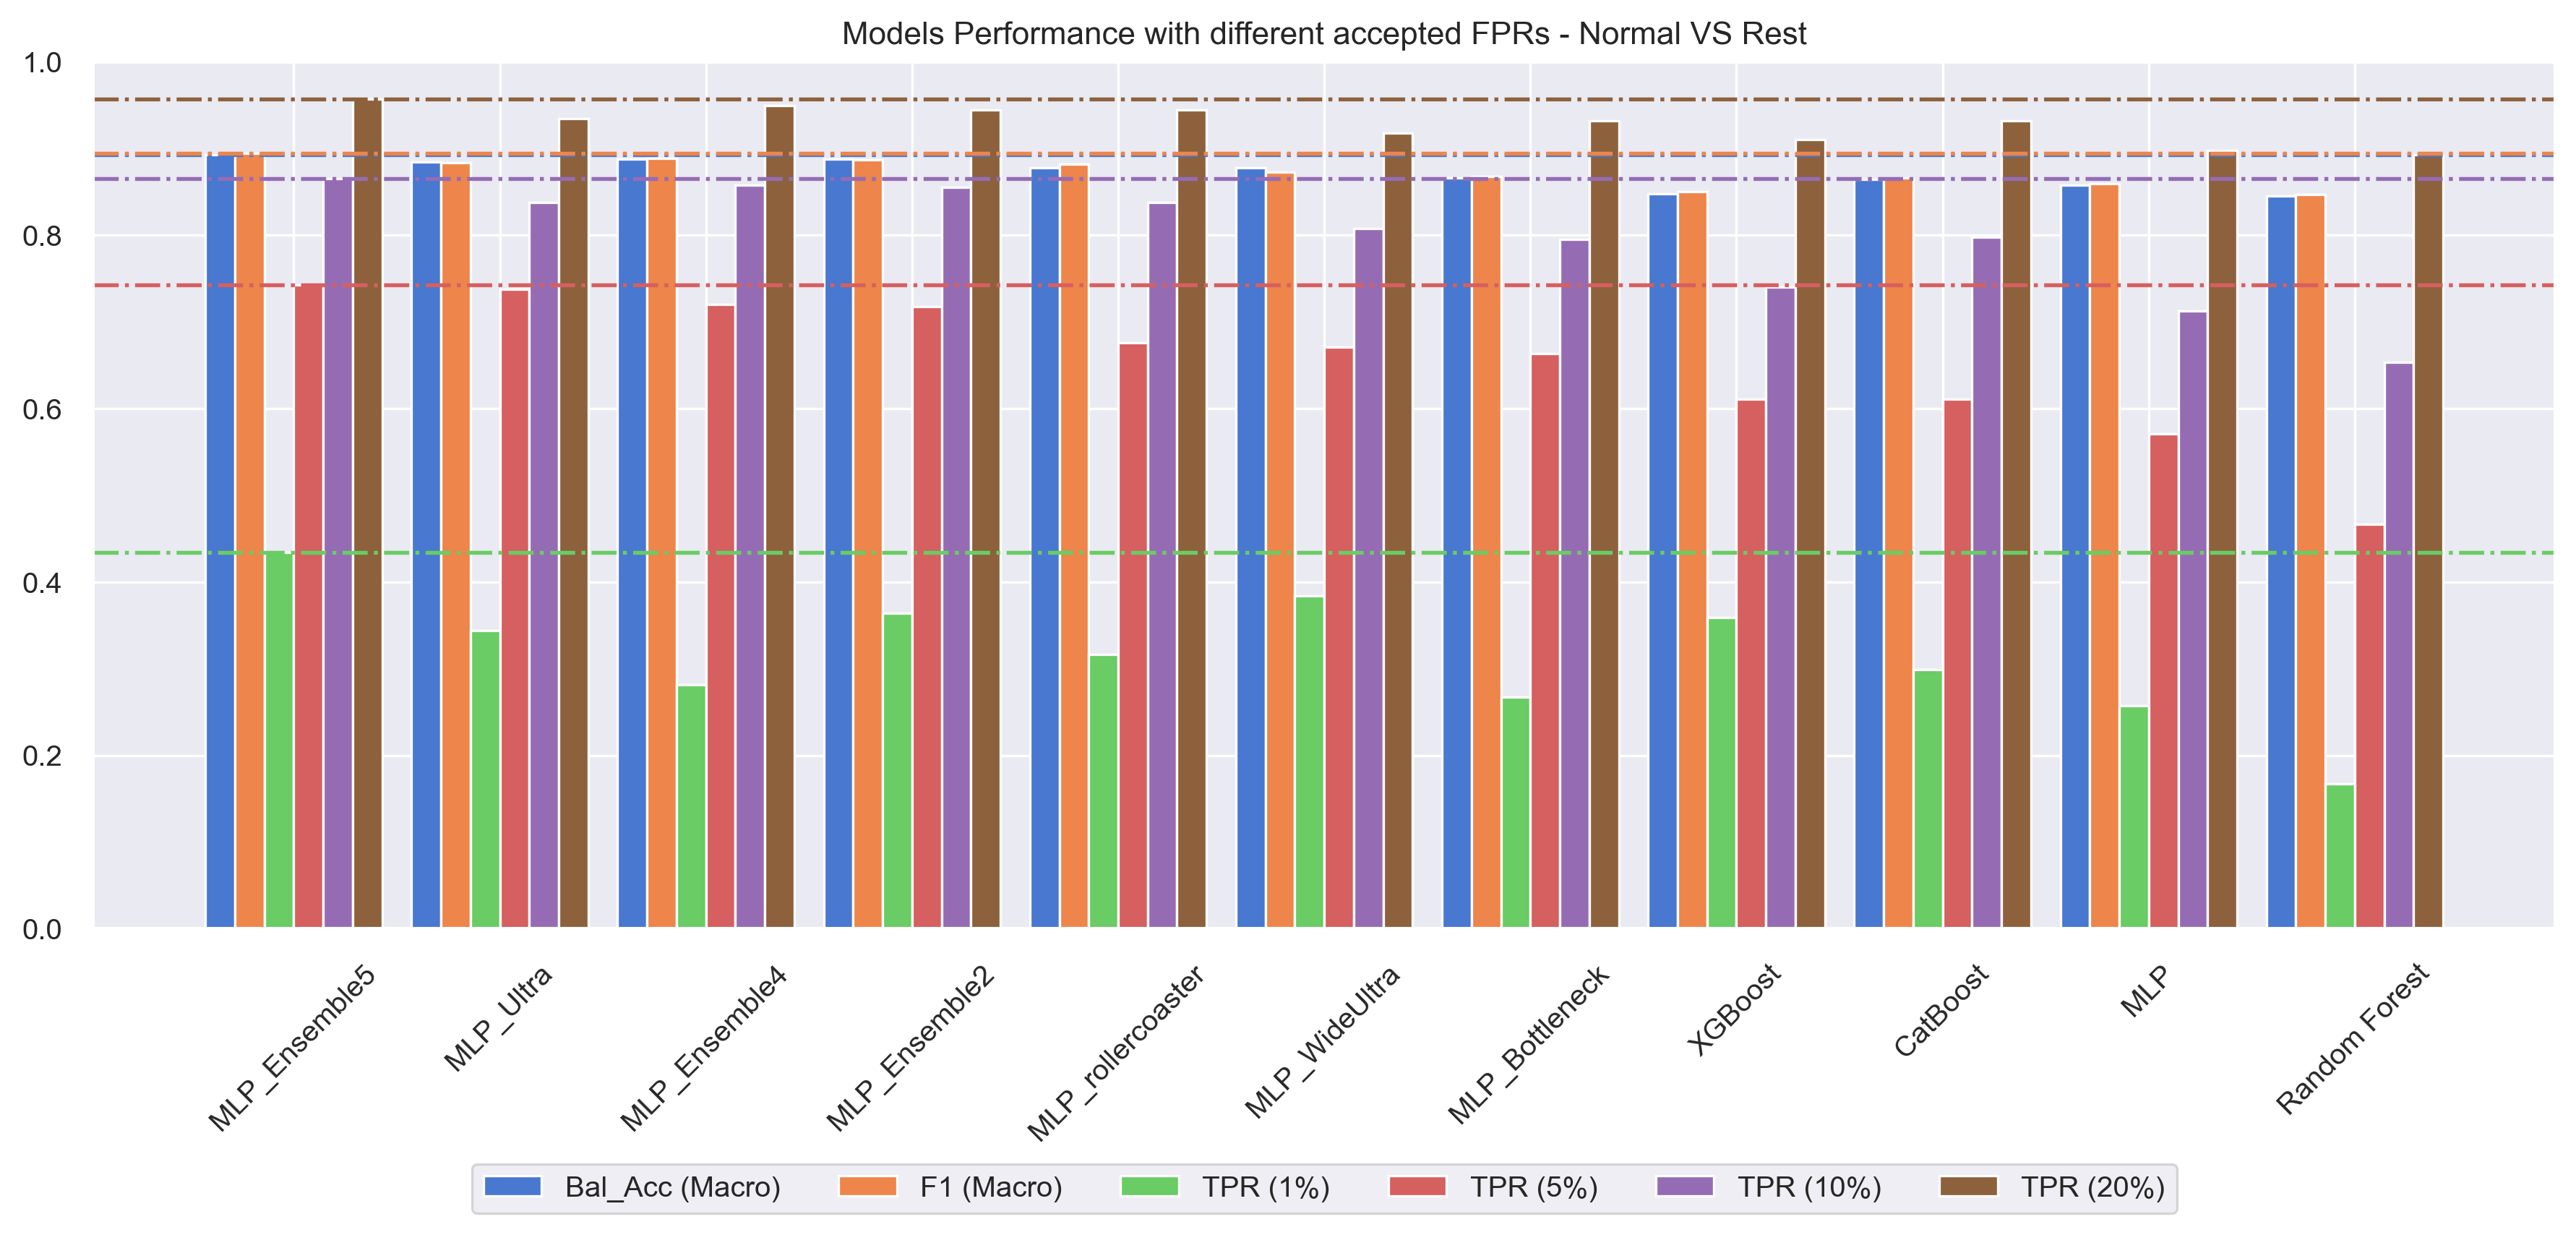
\includegraphics[width=1\textwidth]{./images/nomrVSrest_all.png}
    \caption{TPR at different FPR levels for all models.}
    \label{fig:normVSrest_all}
\end{figure*}

At each FPR level, \textit{MLP\_Ensemble5} outperformed the other models, 
achieving TPRs of 43.4\%, 74.3\%, 86.6\%, and 95.8\% at the 1\%, 5\%, 10\%, and 20\% FPR levels, 
respectively. Excluding \textit{MLP\_Ensemble5}, the best-performing model varied by 
FPR level: \textit{MLP\_WideUltra} at 1\%, \textit{MLP\_Ultra} at 5\%, \textit{MLP\_Ensemble2} at 10\%, 
and \textit{MLP\_Ensemble4} at 20\%.

These outcomes highlight the task's challenges in creating a model that performs well across all FPR 
levels and demonstrate the efficacy of a well-built ensemble model, which leverages the strengths of 
different models to achieve optimal performance.

\subsubsection{Best Model Analysis}
%confmat of the models composing it vs confmat of the ensemble


